\subsection{GAD Generative Models} \label{Sec:G}
Generative models for group anomaly detection   assume that data is generated from an underlying statistical process involving observed data variables $\bf X$,  latent variables $\mathcal{H}$ and model parameters $\Theta$.   Hidden or latent variables are introduced to capture the unseen interaction between observed  data variables. Generative methods in topic modeling applications infer  latent statistical properties representing topics in documents.  Usually structural values such as the number of latent variables is selected prior to model inference. % whereas model parameters  control the distribution for a data generating process.
A group anomaly is characterised by irregular proportions of inferred  variables. %We will explain generative models for detecting anomalous groups in the application of topic modelling. 
Table \ref{Notation} summarises the topic modeling  terminology and notation relating to generative models for detecting group anomalies. 


 
% Another important aspect are the  structural parameters that control the number of latent variables in the data generating process.


% ADVANTAGES/ Disadvantages
%The output of generative models is scores however
%scores can be converted into a classification of normal and anomalous groups. Anomalous groups are selected by the top $L$ scores. This is equivalent to defining a threshold value based on the top percentile of scores. Thus a common issue with generative models is that the selection of $L$ is equivocal and context-dependent.
% are  also sensitive to their initial conditions- inference 
 

 

%ADD TO A DIFFERENT SECTION!
%To hand structured groups, more comprehensive models such as Hidden Markov Models and Conditional Random Fields may be applied.

%The desnity of 
%point-based
%distribution-based
 




 \begin{table}[h]
\begin{center}
 	\renewcommand{\arraystretch}{0.98}
 	\tabcolsep=0.2cm 
 \scalebox{1}{
\begin{tabular}{ ccl%lp{45mm}p{45mm}p{45mm}
} 
 \hline\\[-2mm]%[-4mm]
%  \multicolumn{3}{l}{ {\bf Algorithm 1 } \, Generative Process of GMM}\\%[-3mm]%[-2mm]%& Assumptions & Strengths & Weakness   \\%[1mm]
Quantities & Symbol & Description \\[1mm]
 \hline \\[-3mm]
 Fixed&$M$ & Number of groups \\
  Values & $N_m$ & Number of words/documents in   $m$th group \\
%$\mathcal{S}$ 
  & $N$& Total number of words/documents   \\[2mm]
\hline \\[-3mm]
 Structural & $K$ & Number of topics \\
Values  &$J$& Types of regular group behaviors\\[2mm]
\hline \\[-3mm]
Observed  & $ X_{mn} $ & The $n$th word/ documents in $m$th group \\
Variables  & $ X_{\cdot,n} $ & The $n$th word in entire corpus$^*$  \\
${\bf X}$& $ Y_{nn'} $ & The connection of the $n$th word with the $n'$th word  \\[2mm]
 %& $ {\bf G}_{m} $ & The $m$th group is a collection of random variables \\[1mm]
% & $\mathcal{C}_{n}$ &  The group indicator of the $n$th  word \\[1mm]
 \hline \\[-3mm]
 &$\theta$ & Parameter of topic distributions\\
     &$\phi$ &  Parameter of word distributions \\%  &$\chi$ 
  Model   &$\gamma$ & Parameter of genre distributions\\
%  \hline \\[-3mm]Variational  Parameters $\Delta$
Parameters   & $\alpha$ & Prior parameter on topic distributions\\
$\Theta$ &$\beta$ &  Prior parameter  on word distributions\\
 & $\eta $ & Prior on group membership distributions \\
 & $\bf B$ & Blockmodel matrix for  connection probabilities    \\[2mm]
 \hline\\[-3mm]
 &$ Z_{mn} $ & Topic  indicator for $n$th word in $m$th group \\
%&$ Z_{\cdot,n} $ & The topic associated with $n$th word in  entire corpus  \\
 Latent   & $ \chi_{m} $ & Genre  indicator for  $m$th group  \\
Variables & $ \theta_{m} $ & Topic probabilities for $m$th group (when priors are introduced)  \\
$\mathcal{H}$  & $ \phi_{m} $ & Word probabilities for $m$th group (when priors are introduced)  \\
& $\tilde{G}_n $ & Group indicator for the $n$th data instance \\
& $\pi_n $ & Group membership probability for the $n$th data instance \\[2mm]
\hline \\[-3mm]
%& $ C_{pq}$ & The link associated with $p$th and $q$th  word \\\hline \\[-3mm]
 \multicolumn{3}{l}{*Model inference is applied to  entire corpus without incorporating group information.} \\ 
\end{tabular}
}
\end{center}
 \caption{Summary of descriptive notation for generative models  in the context of topic modeling. }
 \label{Notation}
\end{table} 

Generative models are explained in terms of four key components as follows: %introduced in Section \ref{Sec:Problem}. 
\begin{enumerate}[1.]

\item Characterisation function $f_1({\bf G}_{train})= \boldsymbol\Theta$: \\   Generative models  infer a set of model parameters $\boldsymbol\Theta$   to characterise a group training set ${\bf G}_{train}=\{{\bf G}_{1},\dots,{\bf G}_{M}\}$. Structural values such as expected number of topics are selected based on the lowest value of Alkaike Information Criteria (AIC) \cite{AIC} 
 or Bayesian Information Criteria (BIC) \cite{BIC}. 
For observed data variables ${\bf X}$ and model parameters $\boldsymbol\Theta$, the
AIC and BIC scores are respectively calculated  by
\begin{align}%\centering
& \hspace{8mm} AIC({\bf X}, \boldsymbol\Theta)=-\ln L({\bf X}| \boldsymbol\Theta)+|
\boldsymbol\Theta | \label{AIC} \\[1mm]
& \hspace{25mm}\mbox{ and} \nonumber \\ 
& BIC({\bf X}, \boldsymbol\Theta)=-\ln L({\bf X}| \boldsymbol\Theta)+\frac{1}{2}|
\boldsymbol\Theta|\, \ln (|{\bf X}|)\label{BIC}
\end{align}
where $L({\bf X}|\boldsymbol\Theta)$ is the likelihood of observed data variables given the model parameters and $|\cdot|$ is the number of elements in a  vector or matrix. 
Gershman and  Blei \cite{NPB} further describe how automated parameter selection for generative models is achieved through Bayesian non-parametrics however this has a relatively greater time and algorithmic  complexity. 
\end{enumerate}



 % the  variational distribution of latent variable $q(h|\Delta)$ and  the posterior distribution in Equation (\ref{pos}). 

 %Blei and Jordan \cite{blei2006variational}
 
 %Variational Inference for Dirichlet Process Mixtures


  
%  offers an accurate estimation of the distribution in Equation (\ref{pos}) however  it has 

 
 
\begin{enumerate}[2.]
\item Characterisation function $f_2({\bf G}_{test})=Z_m$: \\ 
For unsupervised approaches, a test set coincides with a training set. We consider the $m$th group as the test set with  ${\bf G}_{test}={\bf G}_{m}$.  Many topic models have been applied to GAD applications. Topic models assume a generative process of data and  infer latent statistical properties such as topic proportions in documents. A topic variable indicates that a word is associated with a particular topic.  The characterisation function of the $m$th group is the inferred topic variable $ Z_m$.  
To obtain topic variables, generative models firstly estimate the posterior distribution of observed data and latent variables under given model parameters with %$\mathcal{H}$,  %is estimated by 
\begin{align}
p({\bf X},\mathcal{H}| \boldsymbol\Theta) \label{pos}
\end{align}
There are two commonly applied methods for inferring latent variables of generative models. %involving Dirchlet processes.  
Monte Carlo Markov Chain (MCMC) methods iteratively  sample from a probability distribution that theoretically converges to the posterior distribution in Equation (\ref{pos}). The equilibrium of a sampled distribution is difficult to assess and has a slow computation especially for larger datasets. Gilks et al. \cite{MCMC} describe different MCMC algorithms for estimating distributions in practice. If applicable, collapsed Gibbs sampling offers a faster computational time for generative models as implemented by Porteous et al. \cite{fastCGS}.


 Another way to infer model parameters   is by   computing an Expectation-Maximisation (EM) algorithm  
  using variational inference. In variational inference, $q(\mathcal{H}|\Delta)$ is a  distribution of latent variables  $\mathcal{H}$ with variational parameters $\Delta$. A variational distribution approximates the  posterior distribution in Equation (\ref{pos}). By  minimizing Kullback-Leibler (KL) divergence between distributions, the optimal variational parameters are computed from 
\[ 
\Delta^* =  \underset {\Delta }{\mbox{argmin}} \;
D_{KL} \Big( p({\bf X},\mathcal{H}|   \boldsymbol\Theta) \,\Big|\Big|\,  q(\mathcal{H}|\Delta) \Big)
\]
where $D_{KL}$ is the KL divergence. For a faster and scalable procedure when dealing with large datasets, stochastic variational inference is proposed by Hoffman et al.    \cite{stochasticVI}    where the posterior distribution in  Equation (\ref{pos}) is approximated by iteratively  updating noisy gradient estimates of the objective function. 
\end{enumerate}
 %For $K$ topics and $T$ themes, this requires a search to minimise the AIC or BIC over $K$ and $T$. 
 
\begin{enumerate}[3.] 
\item Measure $ \mathcal{D}\big(f_1({\bf G}_{train}), f_2({\bf G}_{test})\big )$: \\
Generative models usually compute likelihood scores  from model parameters to determine which groups exhibit a higher degree of anomalous activity.  
 The anomalous behavior of a test group ${\bf G}_{m}$ is  quantified by the negative log-likelihood score
 \begin{align}
 \mathcal{S} ({\bf G}_{m}) = - \ln P({\bf G}_{m} | \Theta) \label{GroupL}
 \end{align}
 The likelihood score in Equation (\ref{GroupL}) is heavily influence by individual outliers and more effectively characterises point-based group anomalies. On the other hand, distribution-based group anomalies are more appropriately quantified by a likelihood score involving topic variables  
\begin{align}
 \mathcal{S} ({\bf G}_{m}|Z_{m}) = - E_{Z_{m}} [\ln P({Z}_{m} | \Theta) ] 
  \label{TopicL}
\end{align}
Since topic variables are latent,  group scores in Equation  (\ref{TopicL}) are estimated through Monte Carlo integration using Gibbs sampling.  
\end{enumerate}

 

\begin{enumerate}[4.]
\item Threshold $\epsilon $ is  selected by domain experts: \\  
Since generative methods only calculate likelihood scores that are relative to a particular dataset, it is difficult to obtain a universal threshold value.  Higher  scores are interpreted as groups with a greater degree of anomalous activities. A threshold is arbitrarily selected based on a proportion of  groups with the highest scores.  In most  generative models, group deviations are associated with  scores that are greater than a subjectively chosen  threshold. Alternatively, it is possible that additional analysis such as a  bootstrapping procedures  provide generative models with a universal  threshold. % for group deviation scores.  
%For a particular supervised generative model by Soleimani \& Miller \cite{ATD} provide 
\end{enumerate} 
%
%\begin{center}
%{\bf General advantages and disadvantages of  generative models}\\ 
%Advantages:
%\begin{enumerate}[(1)]   \setlength\itemsep{5pt}
%\item     Due to their flexible structure,   generative models are able to incorporate prior knowledge
%\item unsupervised learning, generative models are useful for anomaly detection applications as  ground truth labels are usually unavailable
%\item Effective results for generative models  are shown  in Xiong et al. \cite{FGM} for examining multiple types of group behavior as well as Yu et al. \cite{GLAD}  for simultaneously clustering data points and detecting group anomalies
%\end{enumerate} 
%Disadvantages:
%\begin{enumerate}[(1)]   \setlength\itemsep{5pt}
%\item     The effectiveness of generative models is dependent on the appropriateness of assumed generative process for a particular dataset
%\item  Results are also sensitive to model selection where model comparison are computational intensive
%\item Compute scores however do not provide a statistical significance. 
%\end{enumerate}
%\end{center} 
%There are many benefits and disadvantages of  implementing  generative models. 
%By applying  unsupervised learning, generative models are useful for anomaly detection applications as  ground truth labels are usually unavailable.  
%  Due to their flexible structure,   generative models are able to incorporate prior knowledge however the effectiveness of results is dependent on the   appropriateness of model assumptions for a particular dataset.  Results are also sensitive to model selection such as specifying structural parameters. %Gershman and  Blei \cite{NPB} provide an tutorial of Bayesian non-parametrics where automated parameter selection for generative models is achieved at the cost of a  greater time complexity.  
% Effective results for generative models  are shown  in Xiong et al. \cite{FGM} for examining multiple types of group behavior as well as Yu et al. \cite{GLAD}  for simultaneously clustering data points and detecting group anomalies.

%  assuming an underlying  data generating process is disadvantageous when  assumptions are not an appropriate fit for a particular dataset.  
  % of distributional information for 
 %observed and latent variables given certain   parameters.     


\subsubsection{Known Groups Memberships}
Firstly we discuss the details of GAD generative models when group memberships are known a priori. Groups of related instances are naturally defined in many applications. For example,  a document is a group of words whereas a corpus is a collection of documents.    
 In topic modeling applications, statistical properties of groups are described in terms of topic proportions. We now highlight similarities and differences between state-of-the-art generative models for detecting group anomalies. % Either way, an anomalous group is characterised by irregular topic mixtures. Multiple regular behaviors are also investigated where the term 'genre' denotes a regular mixture of topic %Since many of the generative models that will be introduced are commonly implemented in NLP, we adapt the and examples to this field of research. 

%Figure \ref{Fig:GenModel} illustrates the general methodology behind generative models. 
%
%\begin{figure}[h]
%\centering
%\includegraphics[width=15cm, height=4cm]%,trim=2cm 5.2cm 1cm 3.5cm]
%{Generative_Models} 
%\caption{The process of the following generative models }
%\vspace{-1cm}
%\label{Fig:GenModel}
%\end{figure}

 % Genre is type of regular behavior


{\it Gaussian Mixture Models}:\\
The Gaussian Mixture Model (GMM) is a commonly used probabilistic generative model in applications from high energy particle physics \cite{GMM} to speaker verification \cite{speakerV}.    
%A Dirchlet distribution 
%Process Gaussian Mixture Model  (DPGMM) \cite{stochasticVI}  
 %  Model parameters of GMM are inferred by a standard Expectation-Maximisation algorithm 
%The GMM structure involves a mixture of weighted Multinomial  distributions  instead of Gaussian distributions for topic modeling applications.  
Figure \ref{Fig:GMMvsLDA} (a) illustrates the generative process of GMM in plate representation. $N$ words in the corpus are assumed to be generated  from $K$ different topic-word distributions. 
Given $K$ topics, a topic variable for the $n$th word is generated from a Multinomial probability with parameter $\theta $ such that $Z_{\cdot,n} \sim \mbox{Multi}(\theta )$.    
 % For large number of topics ($K \to \infty$), a standard GMM overfits data so DPGMM introduces a Dirichlet prior where $\theta \sim \mbox{Dir}(\alpha)$. 
% The probability that a word is associated with a particular  topic is given by  $ p({X_n}|\beta_{Z_{\cdot, n}})$.  
% $Z_m$ then the density is $ p({X_n}|\beta_{k}) =N({X_n}|\mu_{k}, \Sigma_{k} )$ for continuous variables. 
The posterior distribution in Equation (\ref{pos}) is based on data variables ${\bf X}= \{ X_{{\cdot},n} \}_{n=1}^N $, latent variables $\mathcal{H}=\{Z_{\cdot,n}\}_{n=1}^N$ and model parameters $\Theta=\{\theta,\phi\}$.  Since GMMs do not incorporate  group information (document context),  model parameters are inferred  over the entire dataset so that GMM detects point-based group anomalies rather than distributed-based group deviations. 
%The  scores for the $m$th document  is calculated using Equation (\ref{GroupL}) where model parameters $\Theta$ are learned by  GMM or DPGMM with 
 

%GMM with a conjugate prior on the topic distribution.
%A  is similar to the next generative model however Figure \ref{} highlights the key difference. %

%\subsubsection{}

{\it Latent Dirichlet Allocation}:\\
 Latent Dirichlet Allocation (LDA) proposed by Blei et al. \cite{LDA} is a  popular and widely used generative model  for topic modelling. Figure \ref{Fig:GMMvsLDA} (b) depicts the generative process of LDA in plate representation. 
Given a particular document (group), a word is generated from one of $K$ topic-word distributions with $Z_{m} \sim \mbox{Multi}(\theta_m )$.  LDA  introduces 
  Dirichlet priors on Multinomial distributions with $\theta_m \sim \mbox{Dir}(\alpha)$  to account for  uncertainty of unknown topic quantities and also prevent  overfitting to a large number of topics  in high-dimensional text data.

%The posterior distribution in Equation (\ref{pos}) is based on data variables ${\bf X}= \{ X_{mn} : n=1,\dots,N \mbox{ and } m=1,\dots,M \} $ and model parameters $\Theta=\{\alpha,\phi\}$. 
 The  posterior distribution using Equation (\ref{pos}) is estimated for observed documents   with 
 \begin{align*}
& \mbox{Observed Data:  \;\; \quad}  {\bf X}= \{{\bf G}_{1},{\bf G}_{2},\dots,{\bf G}_{M} \}\\
 & \mbox{Latent Variables: \quad}    \mathcal{H}=\{\theta_{m},Z_{m} \}_{m=1}^M  \\
 & \mbox{Model Parameters: \;\,}  \Theta=\{\alpha,\phi\} 
 \end{align*} 
   where ${\bf G}_{m} = \{ X_{mn} \}_{n=1}^{N_{m}}$ represents a group is a document of words.    
 
 
% Algorithm 1 and 2 respectively describe the  generative processes of GMM and LDA.
  A key difference in LDA compared to GMM is  the ability to incorporate a hierarchical structure due to document (group) information. This is illustrated in Figure \ref{Fig:GMMvsLDA} where observed variables are given by $X_{mn}$ in LDA which takes accounts for document context rather than fitting over all of the observed words $X_{\cdot,n}$ in GMM.  %The number of words within a document in LDA  can also be modeled by a Poisson distribution however we do not include this in our analysis.  
As there are many extensions of LDA, we focus on generative models that  specifically relate to  GAD. % \cite{ }discovers anomalous documents
The Dirichlet distribution in LDA reduces potential overfitting however since a Dirichlet prior is a uni-modal distribution,  a single optimal topic mixture is fitted for all documents. LDA detects point-based and  distributed-based group anomalies however  it cannot capture multiple types of regular group behaviors.



\begin{figure*}[!t]
    \centering
      \begin{subfigure}[H]{0.8\textwidth}
        \centering
        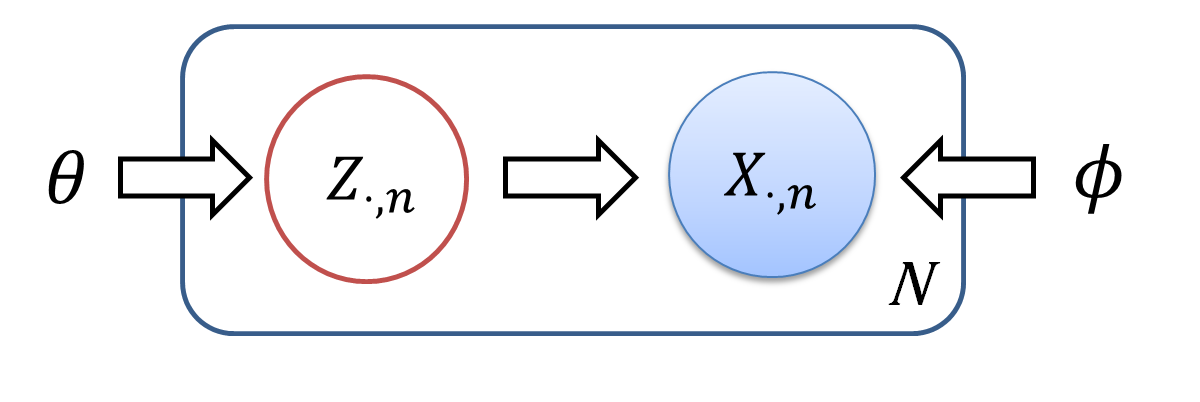
\includegraphics[width=0.75\linewidth, height=2.8cm,
        trim=0cm 0.2cm 1cm 0cm]{FIGURES/GMM}
        \caption{Plate representation for GMM }
    %\vspace{-8mm}
    \end{subfigure}
    \begin{subfigure}[H]{0.8\textwidth}
        \centering
        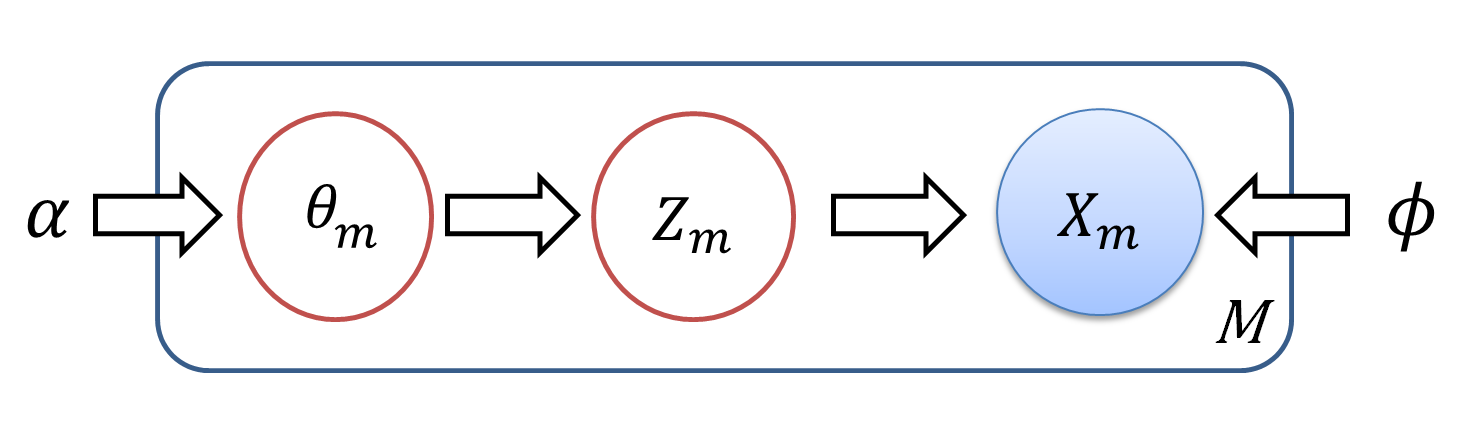
\includegraphics[width=0.9\linewidth, height=3.2cm,
        trim=0cm 0.5cm 1.2cm 0cm% height=1.2in0.75\textwidth% height=1.2in
        ]{FIGURES/LDA}
        \caption{Plate representation for LDA }
       % \vspace{-1.2cm}
    \end{subfigure}% ~   
    \caption{ Plate representation for  Gaussian Mixture Model (GMM) and Latent Dirichlet Allocation (LDA).
Shaded blue circles are observations, circles with red outlines are latent variables and symbols without circles are model parameters. %The blue rectangular plate represents  model is inferred at   particular structural level.
     }
     \label{Fig:GMMvsLDA} 
\end{figure*}



%\begin{figure}[h]
%\centering
%\includegraphics[width=8cm, height=2.5cm, trim=0cm 0.5cm 0cm 0cm]
%{LDA} 
%\caption{Graphical Representation of Latent Dirichlet Allocation (LDA) }
%%\vspace{-2cm}
%\label{Fig:LDA}
%\end{figure}



%The generative process of LDA in Algorithm 2  is similar to GMM however LDA incorporates a hierarchical structure of document information. LDA is described for discrete input data however it can also be adapted for continuous variables.    %To  highlight the key difference of hierarchical structures, Figure \ref{Fig:Compare} illustrates plate representations of both models.
 %A document is a group of words in both models where  regular topic behaviors are inferred for each document in LDA  rather than learning  parameters over the entire corpus in GMM. 
%ncorporates the hierarchical structure of documents
%
% \begin{table}[h]
%\begin{center}
% 	\renewcommand{\arraystretch}{1.1}
% \scalebox{1}{
%   \parbox[h]{5cm }%{.5\lineheight}
%   {
%   \medskip
%   \medskip
%\begin{tabular}{ p{38mm} } 
% \hline\\[-4mm]%[-4mm]
%  {\bf Algorithm 1:}   Generative %\\
%  Process of GMM  \\[1mm]
% \hline \\[-3mm]
% Assume topics $Z_{\cdot, n} \in \{1,\dots, K\}$.\\
%%  Topic weight $\theta \sim \mbox{Dir}(\alpha)$\\
%  {\bf for} word $n=1$ to $N$: \\[1mm]
%\quad (a) $Z_{\cdot n} \sim \mbox{Multi}(\theta )$ \\ %_{n}
%\quad (b) $ X_{\cdot n}\sim p({X}_{\cdot n}|\phi_{Z_{ \cdot, n }})  $\\[1mm]
%{\bf end for}\\[2mm]
% \hline\\[-2mm]
%%A Dirichlet prior may also be introduced on topic probabilities. 
%\\
%\end{tabular}
%}
%\quad % \vspace{-2mm}
% 	\renewcommand{\arraystretch}{1.2}
%   \parbox[h]{5cm }%{.5\lineheight}
%   {
%\begin{tabular}{ p{60mm} } 
% \hline\\[-3mm]%[-4mm]
%  {\bf Algorithm 2:}   Generative Process of LDA \\%[-2mm]%& Assumptions & Strengths & Weakness   \\%[1mm]
% \hline \\[-4mm]
% Assume topics $Z_{mn} \in \{1,\dots, K\}$.\\
%  {\bf for} document (group) $m=1$ to $M$: \\
%\qquad  Topic weight   $ \theta_{m} \sim \mbox{Dir}(\alpha)$ \\
%\qquad    {\bf for} word $n=1$ to $N_m$: \\
%\qquad\quad (a) $Z_{mn} \sim \mbox{Multi}(\theta_{m})$ \\
%\qquad\quad (b) $ X_{mn}\sim p({X}_{mn}|\phi_{Z_{mn }})  $\\
%\qquad {\bf end for}\\
%{\bf end for}\\[1mm]
% \hline\\[-2mm]
%%A Dirichlet prior may be introduced on topic probabilities as $\alpha \sim Dir( \theta)$. \\ 
%\end{tabular}
%}
%}
%\end{center}
%\end{table} 
 





%Both GMM and LDA calculate an anomalous score for each group. However the inferred model for LDA also incoporates the group information. The likelihood score based on topic mixtures given the inferred model parameters is calculated
%using (\ref{TopicL}). 


 %A score for the group behavior is calculated

%  Even though LDA may original proposed for discrete data from frequency word counts, it is easily extended for real-valued continuous data. The points in this case are generated by Gaussian distributions  $p(x|z,\phi)= N(x|\phi_z)$ where $\phi_k =\{\mu_k,\Sigma_k\}$. 
%MGM



%\subsubsection{}

{\it Mixture of Gaussian Mixtures (MGM)}:\\
 To overcome shortcomings of LDA, MGM is proposed by   Xiong et al. \cite{MGM} for distinguishing multiple types of group behaviors. % where MGM refers to Mixture of Gaussian Mixtures whilst for discrete features MGM is the Multinomial Genre Model.
  MGM is an adaption of  Theme Topic Mixture Model (TTMM) %proposed by  Keller  and Bengio 
  \cite{TTMM}  where instead of discrete datasets, MGM is constructed for continuous real-valued input data.  The MGM model introduces genres (themes) as mixtures of topics where each document is associated with certain genres.   %assumes% a group is a collection of documents where 
%  group memberships (collection of documents) are known a priori. 
  For example, books are naturally classified in terms of genres such as sci-fiction, romance, thriller and so on. Given a particular genre (regular group behavior), an anomalous group is characterised by an irregular mixture of topics.  %For $M$ groups, the $m$th group is specified by random vectors $ {\bf G}_{m}=\big\{ X_{mn}  \big\}_{n=1}^{N_m} $. 


In MGM, a document is  categorised by one of $J$ genres and a word in a document is generated from one of $K$ topics.   More specifically, the $m$th document is associated with latent variables such as genres $\chi_{m}$, genre mixtures $\theta_{m}$ and topics $Z_m$. 
The distributional parameters for topics, words and genres are respectively denoted with $\alpha,\phi,\gamma$. 
%is generated by $\chi_{m} \sim \mbox{Multi}(\gamma )$ with $\chi_m \in \{1,2,\dots,J \}$ while a topic from one of $J$ genre has $Z_m \sim \mbox{Multi}( \theta_m )$ where $\theta_m = \alpha_{\chi_m}$.
 The  posterior distribution in Equation  (\ref{pos})   for MGM is expressed as %   ${\bf X}= \{{\bf G}_{m},\dots,{\bf G}_{M} \} $ and model parameters are $\Theta=\{\alpha,\phi,\gamma\}$. 
 \begin{align*}
& \mbox{Observed Data:  \;\; \quad}  {\bf X}= \{{\bf G}_{1},{\bf G}_{2},\dots,{\bf G}_{M} \}\\
 & \mbox{Latent Variables: \quad}    \mathcal{H}=\{\chi_{m},\theta_m, Z_{m} \}_{m=1}^M  \\
 & \mbox{Model Parameters: \;\,}  \Theta=\{\alpha,\phi,\gamma\}
 \end{align*} 
  where ${\bf G}_{m} = \{ X_{mn} \}_{n=1}^{N_{m}}$ represents a group as a collection documents.  
  

We emphasise that in MGM, $  X_{mn} $ represents the $n$th document in the $m$th group rather than the LDA definition of the $n$th word in the $m$th document.   MGM is useful for modeling multiple groups of documents whereas a single document is a group of words for LDA.  
The MGM model also effectively learns multiple types of regular group behaviors however it may  fail to detect   point-based group anomalies  as it does not capture uncertainty of topic-word distributions. Without   Dirichlet prior distributions on topic-word probabilities in MGM, individual anomalies (specific anomalous documents) are poorly detected. 
 
 
 

 %has an identical structure to  %with the additional of a Dirichlet prior on the topic weights. %The TTMM is a simplified version of FGM without topic-group weights. 
%Since TTMM is constructed in the context of document representation, we instead focus on the MGM model as it is applied to group anomaly detection.



%This idea is useful for modeling group-level behaviors but fails to capture anomalous point-level behaviors


%Here we assume there are $K$ topics and $T$ genres. Words from documents are iid from one of $T$ genres with different topic mixtures rather than a single distribution.  A genre $y_i$ is generated from the multinomial distribution $Multi(\alpha)$ and the topic mixtures are dependent on the genres as
%$z_{m,n} \sim Multi(\gamma,y_i)$.  Scores are calculated for each group. MGM assumes a data generating process that does not include
%Dirichlet distributions. 
 
 %Genres are generated from a multinomial distribution where the topics are assigned to each word 


%The dynamic extension of generative models that account for multiple types of normal behavior may be useful to account for seasonal trend in group data.

%A disadvantage of the topic distribution is uni-modal or has a peak at a single point because of the  Dirichlet prior. This behavior cannot capture more multiple types of normal group behaviors.
% Fix this applying KNN clustering the topic weights inferred by LDA however it does not detect the desired anomalies. 
%To extend LDA for multi-model distributions,  from Li (2001) 
%\subsubsection{ThM}
%Since MGM only assumes a data generative process involving multinomial distributions, it does not capture the uncertainty of topic distributions. The Theme Model (ThM) \cite{ThM} assumes a Dirichlet prior on the topic mixtures. The rest of the generative process of ThM is similar  to MGM.
%


%A genre is drawn from a multinomial distribution $y_i \sim Multi(\alpha)$ however topic mixtures are generated from $\theta_i \sim Dir(\alpha_{y_i})$.  The rest of the assumed data generative process is identical to MGM. ThM was originally adapted for discrete data however MGM applies it in 

% \begin{table}[H]
%\begin{center}
% \scalebox{0.95}{
%\begin{tabular}{ p{58mm} p{45mm}} 
% \hline\\[-4mm]%[-4mm]
%  {\bf Algorithm 3}:  Generative Process of MGM \\%[-2mm]%& Assumptions & Strengths & Weakness   \\%[1mm]
% \hline \\[-2mm]
% Assume topics $Z_{\cdot n} \in \{1,\dots, K\}$ and themes $Y_{m} \in \{1,\dots, L\}$ .\\
%  For group of documents  $m=1$ to $M$: \\[1mm]
%  \qquad 1. Theme $Y_m  \sim\mbox{Multi}(\gamma)$\\
%\qquad   2. Topic weight   $ \theta_{m} \coloneqq \alpha_{Y_m}$ \\
%\qquad  3.   For word $n=1$ to $N_m$: \\
%\qquad  \quad (a) $Z_{mn} \sim \mbox{Multi}(\theta_{m})$ \\
% \qquad\quad (b) $ X_{mn}\sim p({X}_{mn}|\,\phi_{Z_{mn } })  $\\[2mm]
% \hline\\[-2mm]
%%A Dirichlet prior may also be introduced on topic probabilities. \\
%\end{tabular}
%\quad\quad
%\begin{tabular}{ p{70mm}p{45mm}p{45mm}p{45mm}} 
% \hline\\[-4mm]%[-4mm]
%  {\bf Algorithm 4}:   Generative Process of FGM\\%[-2mm]%& Assumptions & Strengths & Weakness   \\%[1mm]
% \hline \\[-2mm]
% Assume topics $Z_{\cdot n} \in \{1,\dots, K\}$ and \\ themes $Y_{m} \in \{1,\dots, L\}$ .\\
%  For group of documents $m=1$ to $M$: \\[1mm]
% \qquad 1.  Theme $Y_m  \sim \mbox{Multi}(\gamma)$\\
% \qquad 2. Topic weight   $ \theta_{m} \sim \mbox{Dir}(\alpha,Y_m)$ \\
% \qquad 3. Topic-group weights $ \{\phi_{m,k} \sim p(\eta_k) \}_{k=1}^K$ \\
% \qquad 4.   For word $n=1$ to $N_m$: \\
% \qquad \quad (a) $Z_{mn} \sim \mbox{Multi}(\theta_{m})$ \\
% \quad\qquad  (b) $ X_{mn}\sim p({X}_{mn}|\,\phi_{m, Z_{mn} })  $\\[2mm]
% \hline\\[-2mm]
%%A Dirichlet prior may be introduced on topic probabilities as $\alpha \sim Dir( \theta)$. \\
%\end{tabular}
%}
%\end{center}
%Additionally the number of  words in a group of documents may follow a Poisson distribution.
%\end{table} 
  
 
 
 
%\subsubsection{}
 

{\it Flexible Genre Model (FGM) }:\\ 
 Xiong et al. extends MGM in a method called Flexible Genre Model (FGM).  Similar to MGM, multiple regular group behaviors are considered where a group or collection of documents is characterised by its topic  mixtures given a specific genre.  In addition, FGM  incorporates the uncertainties  of topic-word probabilities.   Dirichlet prior distributions in FGM account for  local document  structures as well as global group information  when estimating the topic-word probabilities.   This results in a better detection of point-based group anomalies as compared to MGM. 
 The topic-group weights are generated from a Dirichlet prior when data is discrete and Gaussian-Inverse-Wishart distributions for continuous real-valued datasets.
 
 Figure (\ref{Fig:FGM}) illustrates the graphical structure of FGM. MGM has a similar representation however it does not include Dirichlet priors on topic-word probabilities with $\phi_m \sim Dir(\beta)$. With  additional Dirichlet priors, the posterior distribution for FGM is identical to MGM  except for additional latent variables  $\{ \phi_m\}_{m=1}^M$ and model parameters in FGM with $\Theta=\{\alpha,\beta,\gamma\}$ rather $\Theta=\{\alpha,\phi,\gamma\}$ in MGM. For an appropriate comparison with MGM, FGM is also formulated for continuous real-valued data however it can also be adapted for discrete or categorical data.   Overall, FGM is more effective than LDA and MGM for modeling multiple types of regular group behavior as well as detecting point-based and distribution-based group anomalies. 


%Algorithm 3 and 4 describe the generative process of MGM and LDA respectively.
%FGM is a more complex model however it has a effective performance for detecting point-based and group-based group anomalies when multiple regular group behaviors are present.
\begin{figure}[H]
\centering
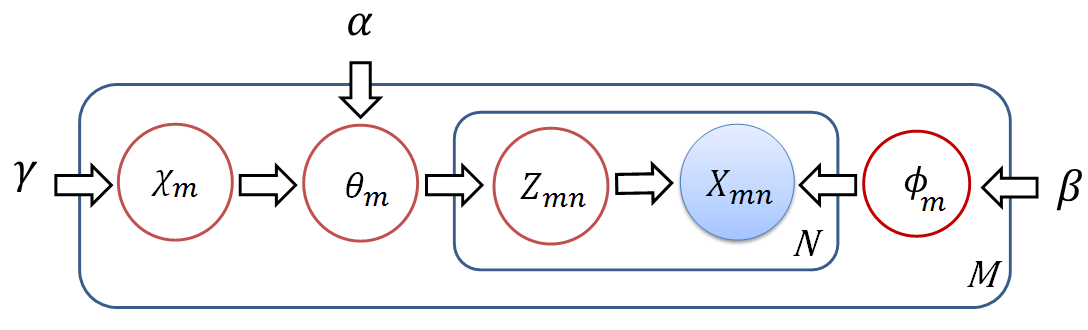
\includegraphics[width=14cm, height=4cm,trim=0cm 0cm 0cm 0.4cm]
{FIGURES/FGM} 
\caption{Graphical Representation of FGM. 
Shaded blue circle contains observed data, unfilled  circles with red outlines are latent variables and symbols without circles are model parameters.}
%\vspace{-2cm}
\label{Fig:FGM}
\end{figure}
 
%The anomalous score of the $m$th group is calculated by $E_{{\bf z}_i }[ -\log   p({\bf z}_i |\Theta) ]$ where $\Theta = \{\pi,\beta\}$. The integration can be computed either by Gibbs sampling or Monte Carlo simulation.

%From Algorithm \ref{Al:LDA}, the points are generated by $x_{m,n}\sim p(x|z,\beta)$. For documents, words are generated with $p(x_{m,n}|z_{m,n}=k,\beta)= Multi(x|\beta_z)$ where $\beta$ is a sparse probability of words occurring in a dictionary list.  A disadvantage of this probability is that  documents globally share the same topics.
 
 
 
 % For example, keywords relating to various topics are learned  keywords from a particular document within the corpus where . 
 %Compared to LDA, FGM allows for more complex group distributions such as the occurrence of multiple types of non-anomalous group behaviors.
 







%\subsubsection{Non-parametric Genre Model (NGM) }


% LDA assumes a document is a group of latent variables called topics then an anomalous document has irregular mixtures. Depending on our definition of a group, a text corpus is a group of documents and anomalies can be detected in a similar way.
 

%Firstly, we introduce the hierarchical Bayes model called . It has been widely used in natural language processing however it can also used for group anomaly detection.
%the points are generated from one of the $K$ topics with $p(x|\alpha)=Multi(x|\alpha,z)$.
% the $n$th point (word) in the $m$th group (document) is distributed by
% More precisely, assume   %

\subsubsection{Unknown Group Memberships}
We now elaborate on details of generative models where group memberships are unknown.   Clustering data instances into groups introduces an additional layer of  uncertainty and may not represent true group structures. Halkidi et al. \cite{ClusterValidity} discuss issues with the validity of clustering techniques %and F\~{a}rber et al. \cite{ClusterEval}  highlight that group labels may not even correspond to natural clustering structures.  
so a careful evaluation and interpretation of inferred clusters is required when true group memberships are unknown. To reduce the uncertainty of clustering data instances, Group Latent Anomaly Detection (GLAD) model \cite{GLAD} incorporates additional information from pairwise connections between data instances. %Yu et al. \cite{GLAD} find that the GLAD model has a relatively higher accuracy for inferring clusters given pointwise and pairwise data.
  Yu et al. \cite{GLAD} demonstrate the effectiveness of  GLAD in grouping data points compared to a number of graph-based clustering algorithms.

%In this way, GLAD simultaneously infers a cluster and detects group anomalies. 
 % and individual features. clusters data based on
%Anomalous Topic Detection (ATD) also infers an anomalous cluster using a generative model however ATD is formulated as an hypothesis test.   %is a supervised method for clustering documents whereas 

% Table \ref{Notation2} introduces additional notation is required for  ATD and GLAD model.


% \begin{table}[H]
%\begin{center}
% 	\renewcommand{\arraystretch}{1.2}
% \scalebox{0.9}{
%\begin{tabular}{ clp{22mm}l%lp{45mm}p{45mm}p{45mm}
%} 
% \hline\\[-4mm]%[-4mm]
%%  \multicolumn{3}{l}{ {\bf Algorithm 1 } \, Generative Process of GMM}\\%[-3mm]%[-2mm]%& Assumptions & Strengths & Weakness   \\%[1mm]
%  Symbol & Description \\%[-3mm]
% \hline \\[-3mm]
% $\mathcal{D}^0$  & Training set \\
% $\mathcal{D}^t$ & Test set \\
% $|\mathcal{D}_m^t|$ & Number of words in the $m$th document \\ 
% $\mathcal{C}$ & Candidate Cluster \\ 
%  $\mathcal{D}^t-\mathcal{C}$& Test set without cluster \\ 
%  $\tilde{G}_{n_1}$ & Group membership of documents $m_1$ \\
% $\tilde{L}_{{n_1},{n_2}}$ & Link between documents $m_1$ and $m_2$ \\
%$B$ & Blockmodel parameter \\   
% \hline\\[-10mm]
%% \multicolumn{3}{l}{*Model inference applied to  entire corpus without incorporating group information.} \\[-6mm] 
%\end{tabular}
%}
%\end{center}
% \caption{Description of notation  in a NLP context. }
% \label{Notation2}
%\end{table} 



%\subsubsection{}
%  The group anomaly detection problem becomes more challenging when memberships of groups are not previously known.  The  hierarchical structure  of GLAD utilises a combination of LDA as previously discussed and Mixed Membership Stochastic Blockmodel (MMSB) proposed by Airoldi et al.  \cite{MMSB}.  Using additional information involving network connections, Yu et al. \cite{GLAD} propose the GLAD model to infer group memberships %from connection data with node-level information
% and simultaneously discover   groups with irregular topic mixtures. GLAD  clusters documents based on similarity of documents as well as  pairwise connections  between documents.   For example, a connection between academic papers may be defined by their citations or a shared authorship.  
% 
% 
%Yu et al. \cite{GLAD} show that GLAD is an effective clustering tool that offers interesting results however improvements are also possible. A general drawback of this method is its input requirements of pairwise  information that may not be readily available. If the graphical structure of GLAD in Figure \ref{Fig:GLAD} is compared to FGM in Figure \ref{Fig:FGM},   certain aspects are neglected by the GLAD model. Firstly, since there is no prior distributions on topic-word probabilities $\phi_m$, GLAD may not be suitable for point-based group anomalies. Also topic mixtures $\theta$ do not have prior distributions such that overfitting may occur if a large number of topics are examined. Compared to FGM and MGM, GLAD does not account for multiple types of regular group behavior. 
{\it Group Latent Anomaly Detection (GLAD)}:\\ 
The group anomaly detection problem becomes more challenging when memberships of groups are not previously known.  The  hierarchical structure  of GLAD utilises a combination of LDA as previously discussed and Mixed Membership Stochastic Blockmodel (MMSB) from Airoldi et al.  \cite{MMSB} to account for pairwise relationships between data points.  Similar to previous generative models, the $m$th group  is characterised by  topic proportions $\theta_{m}$ and an anomalous group is characterised by irregular topic proportions. % Yu et al. \cite{GLAD} demonstrate the effectiveness of  GLAD in clustering and  discovering group anomalies compared to a number of graph-based clustering algorithms.
 The GLAD model is formulated for discrete data and a general drawback of this method is its input requirements of pairwise connection information that is not readily available. 

The  graphical structure for the GLAD model illustrated in Figure \ref{Fig:GLAD} is noticeably different to FGM in Figure \ref{Fig:FGM}. Firstly without  prior distributions on topic-word probabilities $\phi_m$, GLAD may not be suitable for detecting point-based group anomalies. Also topic mixtures $\theta$ do not have prior distributions such that overfitting may occur if a large number of topics are examined. Compared to FGM and MGM, GLAD   does not account for multiple types of group behavior. % Algorithm 3 further describes the  generative process of GLAD where
In Figure \ref{Fig:GLAD}, 
  ${\tilde G}_{n}$ represents a group membership indicator for the $n$th document with group membership  probability $\pi_n$. Topic variables $Z_n$ are inferred for each data point given their group membership.    The blockmodel parameter $\bf B$ contains  probabilities that documents in different groups share a connection. % one group has a connection with a document from another group. 
GLAD assumes discrete feature data  $ X_{n}$ and connection data $Y_{n n'} \in \{0,1\}$  are respectively generated by  multinomial and Bernoulli distributions. Bernoulli probabilities represent the probability that there is a connection between the $n$th and $n'$th document.% $ X_{n}\sim  \mbox{Multi}({X}_{n}|\,\beta_{Z_{n} })  $ and $ Y_{n n'}\sim \mbox{Bernoulli }( {\tilde G}_{n}^T \, {\bf B} \, {\tilde G}_{n'} ) $. 
   %The group membership  probability $\pi_n$ indicates the likelihood that the $n$th document belongs to a particular group with a Dirichlet parameter $\eta$. 

 The  posterior distribution %in Equation  (\ref{pos})   
$p({\bf X},\mathcal{H}| \boldsymbol\Theta) $ 
 for GLAD has %is summarised as %   ${\bf X}= \{{\bf G}_{m},\dots,{\bf G}_{M} \} $ and model parameters are $\Theta=\{\alpha,\phi,\gamma\}$. 
 \begin{align*}
& \mbox{Observed Data:  \;\; \quad}  {\bf X}= \{{\bf X}_{n} \}_{n=1}^N \mbox{ and } {\bf Y} =\{Y_{nn'}: 1 \le n,n' \le N \} \\
 & \mbox{Latent Variables: \quad}    \mathcal{H}=\{\pi_{n},\tilde{G}_n, Z_{n} \}_{n=1}^N  \\
 & \mbox{Model Parameters: \;\,}  \Theta=\{\eta,{\bf B},\theta, \phi\}
 \end{align*} 
  where the $n$th document is associated with one of $M$ groups with $\tilde{  G}_{n}  \in \{1,2,\dots,M\}$. 
  

%Figure \ref{Fig:GLAD} depicts the graphical representation of GLAD which is slightly different from previous models. Algorithm 3 further describes the  generative process of GLAD where $Y_{n n'} \in \{0,1\}$ represents connections between two documents  and ${\tilde G}_{n}$ is the group membership indicator for the $n$th document. Another important aspect of the GLAD model is the blockmodel parameter $\bf B$ that represents  a matrix of Bernoulli probabilities capturing interactions between documents.  The specific entry $B(m,m')$ represents the probability that a document within the $m$th group has a connection with a document from the $m'$th group. GLAD assumes  connection data is generated by $ Y_{n n'}\sim \mbox{Bernoulli }( {\tilde G}_{n}^T \, {\bf B} \, {\tilde G}_{n'} ) $. The group membership  probability $\pi_n$ indicates the likelihood that the $n$th document belongs to a particular group and has a Dirichlet prior with parameter $\eta$. Similar to previous models, the $m$th group  is characterised by  topic proportions $\theta_{m}$ and an anomalous group is characterised by irregular topic proportions. 


% 
%
% \begin{table}[H]
%\begin{center}
%	\renewcommand{\arraystretch}{1.2}
% \scalebox{1}{
%\begin{tabular}{ l} 
% \hline\\[-4mm]%[-4mm]
%  {\bf Algorithm 3:}  Generative Process of GLAD\\ 
% \hline \\[-4mm] \hline  \\[-4mm]
% Assume groups ${\tilde G}_{n} \in \{1,\dots, M\} $ and  topics $Z_{n} \in \{1,\dots, K\}$. \\ 
%    {\bf for} document $n=1$ to $N$: \\[1mm]
% \quad  Draw Membership Weights  $ {\pi}_{n} \sim \mbox{Dir}(\eta )$ \\
% \quad  Group Indicator   $ {\tilde G}_{n} \sim \mbox{Multi}(\pi_{n} )$ \\[1mm]
% \qquad 2. Topics $R_{n} \sim \mbox{Multi}(\theta_{n})$ \\[1mm]
% \quad   {\bf for} document $n'=1$ to $N$: \\
% \quad   \quad   $ Y_{n n'} \sim \mbox{Bernoulli}( {\tilde G}_{n}^T \,{\bf  B} \, {\tilde G}_{n'} ) $ \\
%\quad  {\bf end for} \\
%\quad  \quad  (a) $ Z_{n}\sim \mbox{Multi}({Z}_{n}|\,\theta_{ {\tilde G}_{n} })  $\\
% \quad \quad  (b) $ X_{n}\sim  \mbox{Multi}({X}_{n}|\,\phi_{Z_{n} })  $\\
% {\bf end for}\\[2mm]
% \hline\\[-2mm]
%\end{tabular}
%}
%\end{center}
%\end{table} 
%\vspace{-5mm}
\begin{figure}[H]
\centering
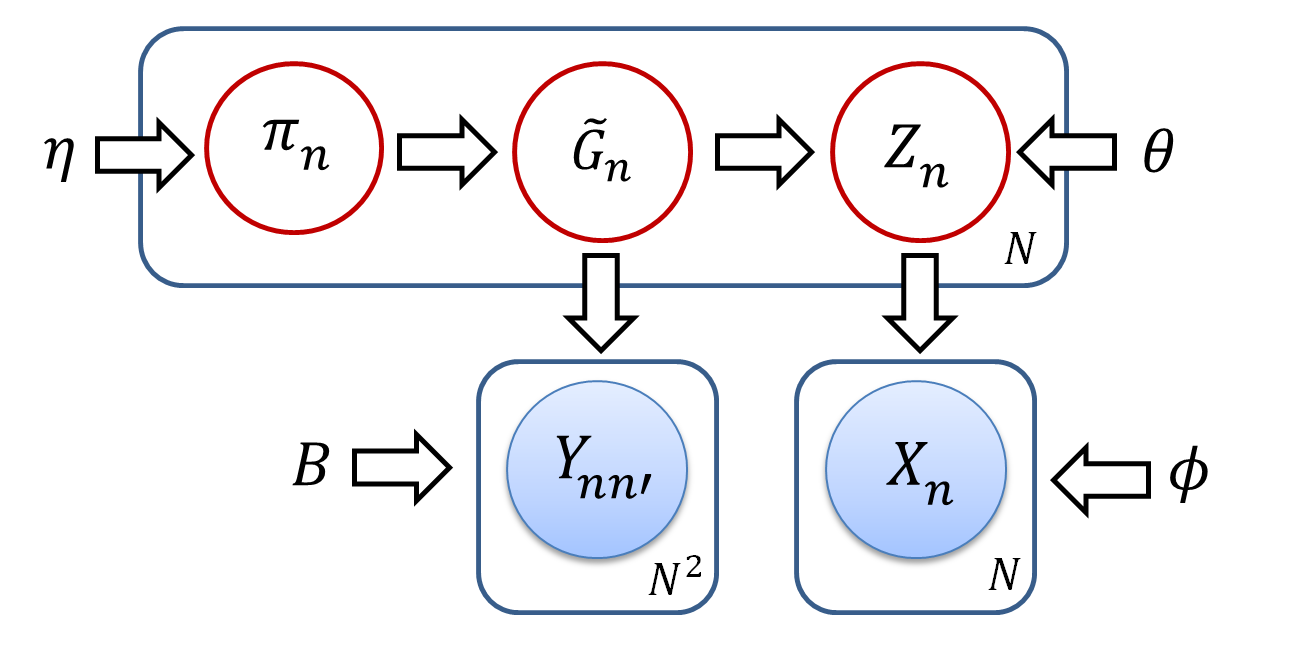
\includegraphics[width=12cm, height= 6cm,trim=0cm 0.6cm 2.5cm 0cm]
{FIGURES/GLAD} 
\caption{Graphical representation of GLAD where shaded blue circles represent observed data, circles with red outlines are latent variables and symbols without circles are model parameters.}
%\vspace{-2cm}
\label{Fig:GLAD}
\end{figure}


 







%\subsubsection{  Multilayer Mixture Model (MLGM)}
%Does not have a hierarchical strucutre.
%{In model-based clustering, the density of each cluster is usually assumed to be a certain basic parametric distribution, for example, the normal distribution. In practice, it is often difficult to decide which parametric distribution is suitable to characterise a cluster, especially for multivariate data. Moreover, the densities of individual clusters may be multimodal themselves, and therefore cannot be accurately modeled by basic parametric distributions. This article explores a clustering approach that models each cluster by a mixture of normals. The resulting overall model is a multilayer mixture of normals. Algorithms to estimate the model and perform clustering are developed based on the classification maximum likelihood (CML) and mixture maximum likelihood (MML) criteria. BIC and ICL-BIC are examined for choosing the number of normal components per cluster. Experiments on both simulated and real data are presented.
%
%Assumes group structure is unknown and perform clustering in the following way.
%$K$ cluster of $J_k$ Gaussian mixtures.
%For example $K=2$ clusters where cluster one consists of $ J_1=4$ Gaussian distributions and $J_2=2$ mixtures. 
%
%The $k$th cluster has the density $\sum_{j \in J_k} b_{k,j} N(x|\mu_j, \Sigma_j)$ and $ \sum_{j \in J_k}  b_{k,j}=1$. The probability density of the whole dataset is 
%\begin{align}
%f(x) = \sum_{k=1}^K \bar{a}_k f_k(x) = \sum_{k=1}^K a_k  \sum_{j =1}^{ J_k}  b_{k,j}N(x|\mu_j, \Sigma_j)
%\end{align}
%%%%%%%%%%%%%%%%%%%%%%%%%%%%%%%%%%%
%%%%%%%%%%%%%%%%%%%%%%%%%%%%%%%%%%%



%Let $\mathcal{D}^0$ and $\mathcal{D}^t$ respectively denote the training data and test set where $|\mathcal{D}_n^t|$ is the number of words in the $n$th document in the test set. The null model is trained on $\mathcal{D}^0$ and estimates $K$ topics in a corpus.


%
%\begin{table}[H]
%\begin{center}
%\begin{tabular}{l  }
%\hline \\
%{\bf Algorithm 3:} Anomalous Topic Discovery (ATD)  \\
%\hline\\[-2mm]
%Input:  Training set $\mathcal{D}^{0}$    and test set $\mathcal{D}^{t}$    \\
%%Learn $\mathcal{M}_0=\{\Theta_0,\Delta_0 \}$ from $\mathcal{D}^{t}$ 
%Compute likelihood under null model for each document in test set \\ $l_0(m) = \ln p (m|\mathcal{D}^0 ) \; \forall \; m  \in  \mathcal{D}^{t}$ 
%\\
%{\bf repeat}%& Calculate ${\bf S}^b =\mbox{score}(\mathcal{D}_b) $ for $b=1,\dots,B$
%\\
%\quad Initialise test cluster $\mathcal{C}=\emptyset$ 
%\\
%\quad Choose document with least likelihood $m^* =  
%\underset {m \in \mathcal{D}^{t} } { \mbox{argmin}}    
% \frac{1}{|\mathcal{D}^t_m| }{ l_0 (m)}$  
%\\
%\quad {\bf repeat}%& \quad $p_1 (S_m) = \frac{1}{U+1}\Big(1+\sum_{u=1}^U I(S_m < \tilde{S}_u)\Big)$
%\\
%\qquad Add document to test cluster $\mathcal{C}  \leftarrow  \mathcal{C} \cup \{m^*\} $%& \quad $p_1 (S_m) < 0.05/m \Rightarrow$ $\hat{\mathbf{G}}_m$ is anomalous 
%\\[1mm]
%%\qquad Learn parameters on	$\mathcal{M}_1=\{\Theta_1,\Delta_1 \}$ from test cluster $\mathcal{C}$  
%\\
%\qquad	Estimate likelihood of documents with $l_1 (m) =\ln p (m|\mathcal{D}^{t} ) \; \forall \; m \in   \mathcal{D}^{t}- \mathcal{C}  $ 
%\\
%\qquad	Compute likelihood ratio  and select 
%  $m^* =\underset {m \in \mathcal{D}^{t}- \mathcal{C} } { \mbox{argmax}}     \frac{l_1 (m) -l_0 (m)} {|l_0 (m)|}		$  
%  
%\\
%\qquad	Test for significance of topic $K+1$ in document $m^* $ $^{ \,\dagger} $    
%\\
%%\qquad \qquad
%%\\
%%\qquad \qquad
%%\\
%\quad {\bf until} Anomalous topic $K+1$ is insignificant in  document $m^*$   
%\\
%%\quad Compute score($\mathcal{C} $) \\
%\quad Test significance of $\mathcal{C} ^{ \; \dagger}$ 
%\\
%\quad Omit cluster from the test set	$\mathcal{D}^{t} \leftarrow \mathcal{D}^{t} -\mathcal{C} $ 
%\\
%  {\bf until} $\mathcal{C}$ is insignificant \\ 
%Output: Anomalous cluster $\mathcal{C}$ with a bootstrap $p$-value \\
%\hline
% \end{tabular}
%\end{center}
%$\dagger$ Full details of bootstrap hypothesis tests for evaluating  statistical significance are described in Soleimani \& Miller \cite{ATD}. 
%\end{table}
 
%\begin{table}
%\centering
%\begin{tabular}{ c  c }
%Test1\tablefootnote{Footnote 1} & Test2\tablefootnote{Footnote 2} \\ 
%\end{tabular}
%\caption{This is a table.\label{FirstTable}}
%\end{table}

%%%%%%%%%%%%%%%%%%%%%%%%%%%%%%%%%%%%%%%%%%%%%%%%%%%%%%%%%%%%


%\subsubsection{Introducing a taxonomy for Generative Models}
% We differentiate the generative methods based on three model parameters $\Theta=\{\alpha,\beta,\gamma \}$ and the length of the chain to their distribution of influence which is denoted by $L_\Theta =L|\Theta, \mbox{variable}(\Theta)|$. More specifically, $ \alpha,\,\beta$ and $\gamma $ are parameter that respectively influence the inferred intragroup variables  (topics), the distributions of the observed features (words) and the inferred multiple types (theme) variables. 
%
%%Firstly, denote the parameter 
%Figure \ref{Fig:LDA} highlights the graphical representation structure of LDA. There are two latent variables, two model parameters and the observed feature vector.
%Using our defined taxonomy,  $\alpha$ is the parameter of the feature probabilities with $L_\alpha=1$. An extension of LDA involves introducing a Dirichlet prior on the feature probabilities such that  $L_\alpha=2$. The Dirichlet parameter $\beta$ influences the topic distributions with a chain length of $L_\beta=2$. More complicated models involve increasing the length of the chain from the model parameters to their latent variables of influence.
%
%
% 
%



%For Multinomial Genre Model (MGM),  $\alpha$  is the $L_\alpha=1$parameter of the feature probabilities, $\beta$ is a Multinomial  parameter that influences the topic distributions and $\gamma$ is the proportion of a specific behavior type. The chain lengths of 
%the hyperparameters to their variable of influence for MGM are
% $L_\alpha=2$, $L_\beta=1$ and $L_\gamma=1$. The graphical structure of Flexible Genre Model (FGM) is illustrated in Figure \ref{Fig:FGM}. The additional inferred variable as compared to MGM, results in the chain lengths   $L_\alpha=2$, $L_\beta=2$ and $L_\gamma=1$ where   $\beta$ is a Dirichlet  parameter.




%LDA is considered as a baseline method in many papers involves group anomaly detection \cite{FGM,MGM}. Algorithm\ref{Al:LDA} describes the generative process of LDA as well as the calculation of the anomalous scores for each group.

%\begin{algorithm}
%    \caption{:  Latent Dirichlet Allocation (LDA) for Group Anomaly Detection}
%  \begin{algorithmic}[1]
%    \INPUT Documents (Groups of Words)  
%    \OUTPUT Group scores based on topic mixtures (distributional measures).
%   %\STATE {\it Generative Process:}
%     \FOR{ Document $m=1$ to $M$}%
%         \STATE      Select topic proportions $ \theta \sim Dir(\pi)$ 
%\FOR{ Words $n=1$ to $N_i$} \\
% Draw topics $z_{m,n} \sim Multi(\theta)$\\
%Generate words $x_{m,n}\sim p(x_{m,n}|{\boldsymbol\beta},z_{m,n})$
%\ENDFOR
%\STATE Calculate score of $m$th group $E_{{\bf z}_i }[ -\log   p({\bf z}_i |\Theta) ]$ where $\Theta = \{\pi,\beta\}$
%\ENDFOR
%  \end{algorithmic} 
%  \label{Al:LDA}
%\end{algorithm}
% 



 
 
 


%\section{Hypothesis Testing}
%A problem with the above methodologies do not provide a significant test when detecting anomalous groups. That means that a detected anomalous group may not be significantly   different. The decision for selecting anomalous behaviors is equivocal and has a degree of uncertainty around it. To quantify the uncertainty of the detected anomalies, hypothesis testing allows for an automated decision making process irrespective of the context.

%\subsubsection{ANOVA}
%Analysis of Variance (ANOVA) is a statistical method for comparing the means of multiple groups.  % Based on chi-square tests $M \time 2 $ tables 
%Assume the group populations are independent. 
%If the group means are not very different, the variation between groups (SSB) will be similar to the variability of the observations within groups (SSW).
%
%Hypothesis is 
%$H_0: \mu_1=\mu_2=\dots=\mu_i$
%vs. $H_1:\mu_i \ne \mu_j $ for $ i,j =1,\dots, M$.
% 
% 
%$F=\frac{MSB}{MSW}$
%
%Multiple Comparisons require Bonferroni adjustments
%
%Chi-square tests are used for comparing binary or categorical data.


%\begin{landscape}
 \begin{table*}[H]
\begin{center}
 \scalebox{0.95}{
\begin{tabular}{ ccp{45mm}p{45mm}p{45mm}p{45mm}} 
 \hline\\%[-4mm]
Method & Data Variables $\bf X$ & Model Parameters $\Theta$ & Strengths & Weakness   \\%[1mm]
 \hline\\%[-4mm]
 LDA & $X_{m,n}$ &  $\alpha, \phi$ & Topic representation & Single topic mixture \\
 MGM & ${\bf G}_{m} $ %=\{X_{m,n} \}_{n} $
    & $\alpha, \phi,\chi$ & Multiple types of group behavior & Cannot detect pointwise anomalies \\
  FGM & ${\bf G}_{m} $  & $\alpha, \beta,\chi$ & detect pointwise anomalies & Complex model \\
  ATD &  ${\bf X}_{m}  $   & $ beta, \phi$ & Incorporates sparse topic variables &  Requires labeled data \\
 %\multirow{2}{*}{GLAD} 
 GLAD & ${\bf X}_{m},{\bf Y}_{m} $   & $\alpha, beta, \psi, B$ & Simultaneously infers groups and detects anomalous groups &  Requires connection data \\
 %  OCSMM &  Group observations are IID  & Flexible representation of group behaviors. Does not require domain knowledge. & Choice of the kernel $k$. Sensitive to the parameter $\nu$ for the expected number of anomalous groups.\\
% KNNG-$\mathcal{D}$ &  Static & KNNG is nonparametric & No interpretation of anomalous group behavior & \\ 
% MQCC & Dyanmic & Group observations are IID.
% Groups are independent over time. &  Requires training data\\
 %LRT & Dynamic & Group observations are IID.
% Groups are independent over time.  & & 
 \\ \hline
\end{tabular}
}
\end{center}
 \caption{Summary of Different Methods}
 \label{Tab:MH}
\end{table*}

%\end{landscape}

